\documentclass[../report.tex]{subfiles}
\begin{document}

\section{Introduction} \label{sec:intro}

The Sokoban game is a challenging single-player game - for both man and machine. Sokoban is a computer puzzle game in which the player pushes jewels around a maze to place them in designated locations. This report describes how to solve the Sokoban game with a minimalistic robot. The LEGO Mindstorms EV3 set \cite{ev3} is used to create the robot.

In this report the Sokoban problem is solved via a hybrid system which is illustrated in \autoref{fig:intro_hybrid}. The solution of the Sokoban map is found separately on a computer and via a "Glue" is the solution translated so the controller on the robot understands what to do. 

\begin{figure}[H]
    \centering
    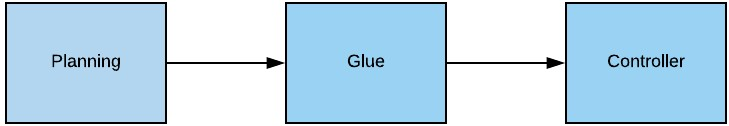
\includegraphics[width=0.75\textwidth]{figures/System_overview.jpg}
    \caption{System overview of the system.}
    \label{fig:intro_hybrid}
\end{figure}

The code for the project can be found at \cite{code}.

\end{document}